\documentclass{article}
\usepackage{graphicx}
 \usepackage{amsmath}
 \usepackage{amssymb}
 \usepackage[parfill]{parskip}


\title{Desmos Polygonal Diagrams (draft)}
\author{Dan MacKinnon}
\date{July 2025}

\begin{document}

\maketitle

\begin{figure}[!ht]
    \centering
    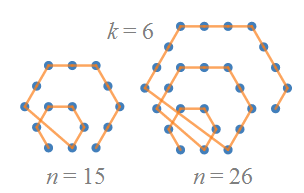
\includegraphics[width=0.5\linewidth]{hexagonal_and_no.PNG}
    \caption{Two hexagonal diagrams, 15 is hexagonal, 26 is not}
    \label{fig:hexagonals}
\end{figure}

Let $n,k \in \mathbb{Z}^{+}$, $n > 2$. We'd like to draw the polygonal number diagram associated with a particular set of of $k$-polygonal numbers for the given number $n$. Figure (\ref{fig:hexagonals}) shows hexagonal number ($k = 6$) diagrams for the numbers 15 and 26. Because 15 actually is a hexagonal number, the diagram is complete. The diagram for 26 shows an incomplete diagram, with an incomplete outer layer.

The layers of a polygonal number diagram are traditionally called \textit{gnomon} layers, with each $k$-polygonal number diagram being made up of a new complete gnomon layer applied to the preceding $k$-polygonal number, as shown in Figure (\ref{fig:gnomons}).

\begin{figure}
    \centering
    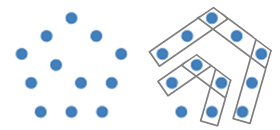
\includegraphics[width=0.5\linewidth]{pentagon_with_gnomon.PNG}
    \caption{Pentagonal number diagram $n=12$ with gnomons}
    \label{fig:gnomons}
\end{figure}


Following this standard approach, to draw up to a given number $n$ in a $k$-polygonal diagram, you determine which gnomon layer it lies in, how far along the gnomon layer it is, and what side of the gnomon it is on. The gnomon layer for $n$ tells us where to start: we just need to count up to the layer along angle that is determined by $k$. If we know how far along in the layer it is, we know how many dots to move along before plotting our point. And finally, if we know which side it is on, we know how many turns to make along the way.

As mentioned, the angle needed in drawing these diagrams is completely determined by which type of polygonal number we are drawing. The shape of the diagram is determined by the angles in a regular $k$-gon. Define $a_{ngle}$ as in equation (\ref{eq:angle}).

\begin{equation}
    a_{ngle}=\left(\pi-((k-2)*(\pi/k))\right)
\label{eq:angle}
\end{equation}


$N$ is the ordered tuple $N=\left[1,\ ...\ ,n\ \right]$. Define the point $\left(x_{kn}\left(N\right),y_{kn}\left(N\right)\right)$ according to the formulas that follow.

\begin{equation}
x_{kn}\left(l\right)=-g_{nomon}\left(l\right)\cos\left(a_{ngle}\right)-\sum_{j=1}^{g_{depth}\left(l\right)}\cos\left(s_{k}\left(j,l\right)\cdot a_{ngle}\right)
\end{equation}

\begin{equation}    y_{kn}\left(l\right)=g_{nomon}\left(l\right)\sin\left(a_{ngle}\right)+\sum_{j=1}^{g_{depth}\left(l\right)}\sin\left(s_{k}\left(j,l\right)\cdot a_{ngle}\right)
\label{eq:yformula}
\end{equation}

The formulas for $x_{kn}$ and $y_{kn}$ express the idea of placing the point corresponding to the current polygonal number at the right spot in the correct gnomon layer for that number, as shown in Figure (\ref{fig:yannotated}).

\begin{figure}
    \centering
    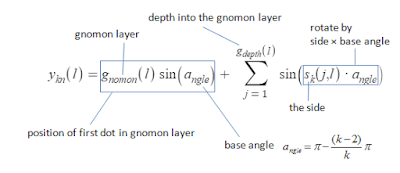
\includegraphics[width=0.5\linewidth]{annotated_eqn.PNG}
    \caption{Formula for $y_{kn}$, annotated}
    \label{fig:yannotated}
\end{figure}


\begin{equation}
s_{k}\left(j,l\right)=\left(\text{ceil}\left(\frac{j}{g_{size}\left(l\right)}\left(k-2\right)\right)+1\right)
\end{equation}

\begin{equation}
g_{size}\left(l\right)=g_{nomon}\left(l\right)\cdot\left(k-2\right)+1
\end{equation}

\begin{equation}
    g_{depth}\left(l\right)=\sum_{o=1}^{l-1}\left(\operatorname{floor}\left(\frac{g_{nomon}\left(o\right)}{g_{nomon}\left(l\right)}\right)\right)
\end{equation}

\begin{equation}
    g_{nomon}\left(l\right)=\sum_{i=1}^{l-1}p_{olygonal}\left(i\right)
\end{equation}

\begin{equation}
    p_{olygonal}\left(l\right)=1-\left(p_{up}\left(l\right)-p_{down}\left(l\right)\right)
\end{equation}

\begin{equation}
p_{down}\left(l\right)=\operatorname{floor}\left(p_{verse}\left(l\right)\right)
\end{equation}

\begin{equation}
p_{up}\left(l\right)=\operatorname{ceil}\left(p_{verse}\left(l\right)\right)
\end{equation}

One method of finding out the gnomon layer we are in is to use a formula for computing polygonal numbers along with the quadratic formula. This approach is expressed in equations (\ref{eq:quadform}) and (\ref{eq:determinant}).

\begin{equation}
    p_{verse}\left(l\right)=\frac{\left(k-4\right)+\sqrt{D\left(l\right)}}{2\left(k-2\right)}
     \label{eq:quadform}
\end{equation}

\begin{equation}
    D\left(l\right)=\left(k-4\right)^{2}+8l\left(k-2\right)
    \label{eq:determinant}
\end{equation}

\section{gnomon commitment}

Comparing the listing for the hexagonal numbers with the diagrams above, you can see how the sequences are built diagrammatically. In general, beginning with a single dot, k-sided polygons are built by adding layers (called gnomons) consisting of k-2 segments, with each segment of the gnomon having one more dot than the segments of the previous layer. In this way, the nth gnomon consists of segments each n dots long, but with k-3 dots shared by adjoining segments (the corners).

\begin{align}
    p_{k, 1} &= 1 \\
    p_{k,n} &= p_{k,n-1} + (k-2)n - (k-3)
\end{align}

\begin{equation}
    p_{k,n} = \sum^{n}_{i=1}\left[(k-2)i-(k-3)\right] 
\end{equation}

\end{document}
